In order to show an improvement on existing predictive simulation systems for CHD corrective surgeries, we want to demonstrate that our blood vessel model based on thin shell elements is
\begin{enumerate}
\item physically accurate, \tomas{I suggest to use "fitness for the purpose"}
\item converges to expected results with a low number of elements,
\item is able to simulate low-level surgical procedures universally.
\end{enumerate}
We close discussion with limitations and constraints of our simulation approach in terms of generation and dynamic remeshing of thin shell element meshes.

A quantitative validation by means of a comparision to real pre- and post-surgery image data is impossible at present. This is mainly due to ethical issues that arise during image data acquirement of infants, i.e. necessary heart rate lowering medications or exposure to radiation. There is no such data available that is obtained shortly after surgeries in infants where the growth of the patient would not interfere comparison. However, a qualitative comparison to real image data acquired months after a surgical intervention, which confirm a principal suitability of predictive simulations for surgery planning, can be found in \cite{Li2009}.

\subsection{Accuracy}

\begin{figure}[tbh]
    \centering
    \begin{tabular}{cc}
     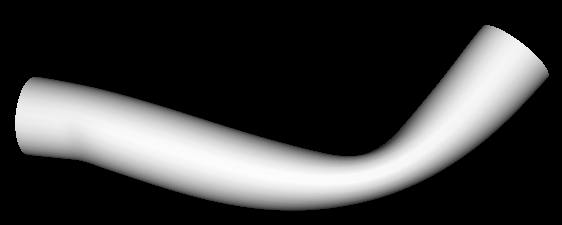
\includegraphics[width=0.3\columnwidth]{img/compare-bend.png}
      &
      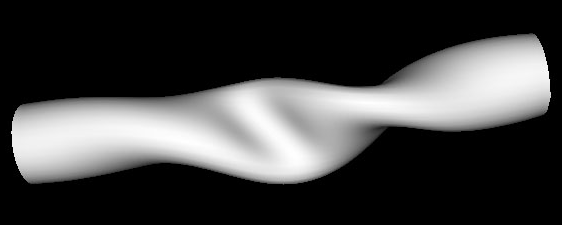
\includegraphics[width=0.3\columnwidth]{img/compare-twist.png}
      \\
      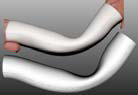
\includegraphics[width=0.3\columnwidth]{img/compare-bend-other.png}
      &
      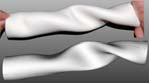
\includegraphics[width=0.3\columnwidth]{img/compare-twist-other.png}
    \end{tabular}
    \caption{Simulation of bending and twisting of an elestic tube. Top row: Thin shell element model; Bottom row: Real elastic tube manipulated by hand and Cosserat rod-based hybrid model\cite{Li2009} (Credits for the bottom images: Li et al.).}
    \label{fig-deformations}
\end{figure}

Figure \ref{fig-deformations} shows bending and twisting of an elastic tube manipulated by hand compared to the simulation results of \cite{Li2009} and our method. These kinds of blood vessel deformations are likely to occur during surgery. Our results are close to the real deformations as expected due to the physically based formulation of thin shell elements.

\subsection{Convergence}

\begin{figure}[tbh]
  \centering
  \begin{tabular}{cccc}
    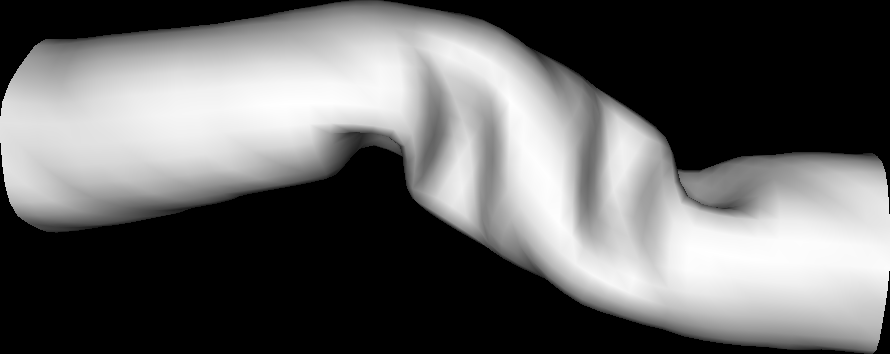
\includegraphics[width=0.24\columnwidth]{img/twist-06-cg.png}
    &
    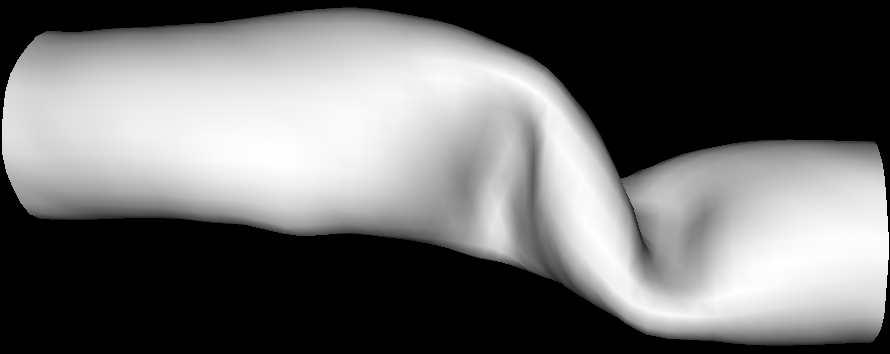
\includegraphics[width=0.24\columnwidth]{img/twist-08-cg.png}
    &
    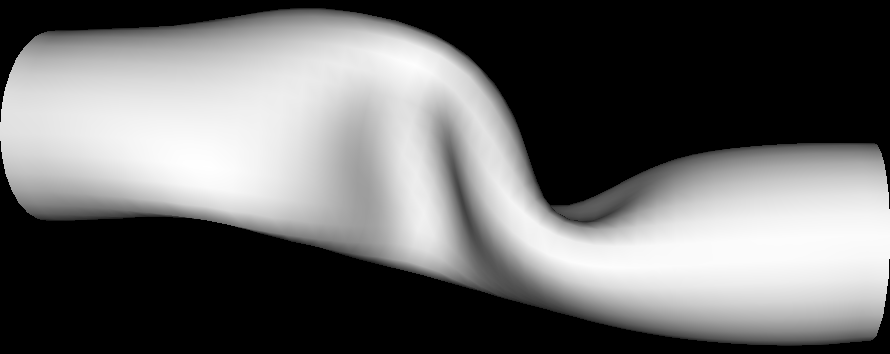
\includegraphics[width=0.24\columnwidth]{img/twist-16-cg.png}
    &
    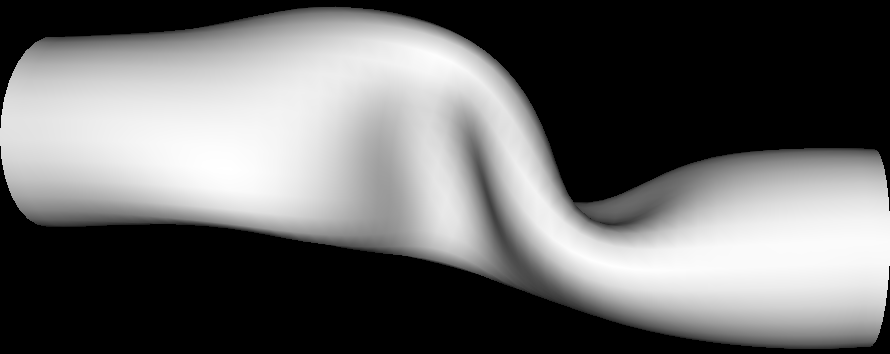
\includegraphics[width=0.24\columnwidth]{img/twist-31-cg.png}
    \\
    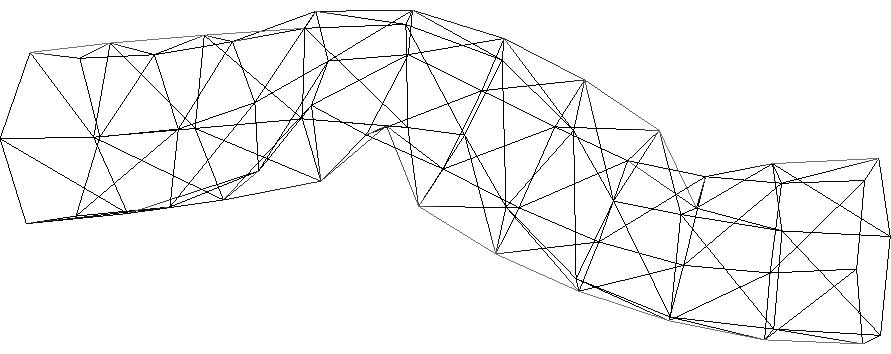
\includegraphics[width=0.24\columnwidth]{img/twist-06w-cg.png}
    &
    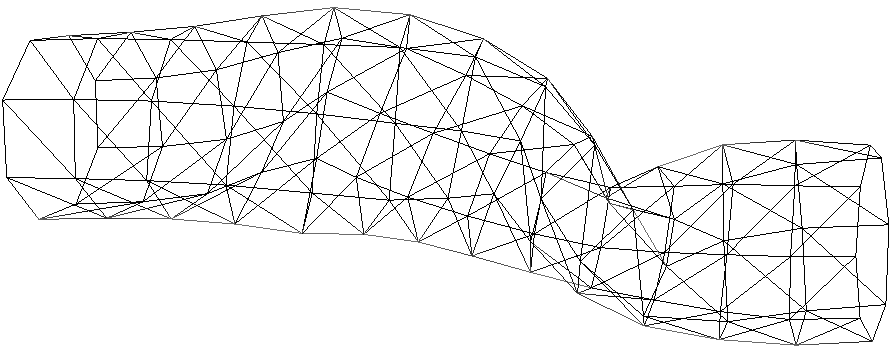
\includegraphics[width=0.24\columnwidth]{img/twist-08w-cg.png}
    &
    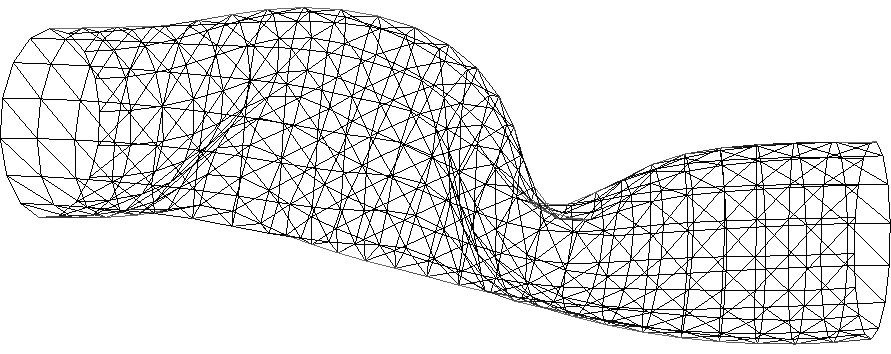
\includegraphics[width=0.24\columnwidth]{img/twist-16w-cg.png}
    &
    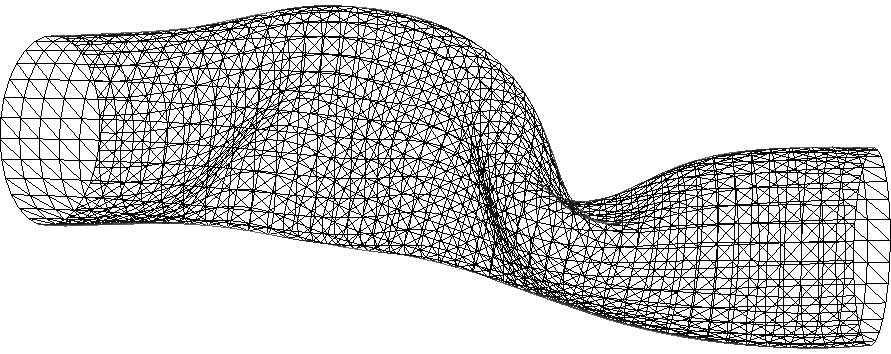
\includegraphics[width=0.24\columnwidth]{img/twist-31w-cg.png}
  \end{tabular}
  \caption{Convergence of a twisted, elastic tube with 6, 8, 16 and 31 vertices
  along its circumference (120, 208, 832 and 3038 thin shell elements). Top row: High polygon count mesh mapped to simulation results of coarser shell element meshes (bottom row).}
  \label{fig-convergence}
\end{figure}

It is important to minimize the number of shell elements to reduce computation time. This is the key factor to enable an interactive simulation system that is accepted by surgeons to simulate multiple surgical approaches in succession. The bending capabilities of thin shell elements allow to reduce their number and still representing the tubular structure of blood vessels while maintaining their physical behavior appropriately. Figure \ref{fig-convergence} shows simulation results of a strongly deformed tube represented by different numbers of thin shell elements. With only eight vertices along the circumference of the elastic tube the simulation result is comparable to a simulation result with high element count. We map a fine polygonal mesh to the coarse shell element meshes to visualize their intrinsic bending detail. \tomas{redundant, already in previous sentences: and therefore to get comparable results that correlates with the true shape of the simulated tube.}

\subsection{Low-level surgical procedures}

\begin{figure}[tbh]
  \centering
  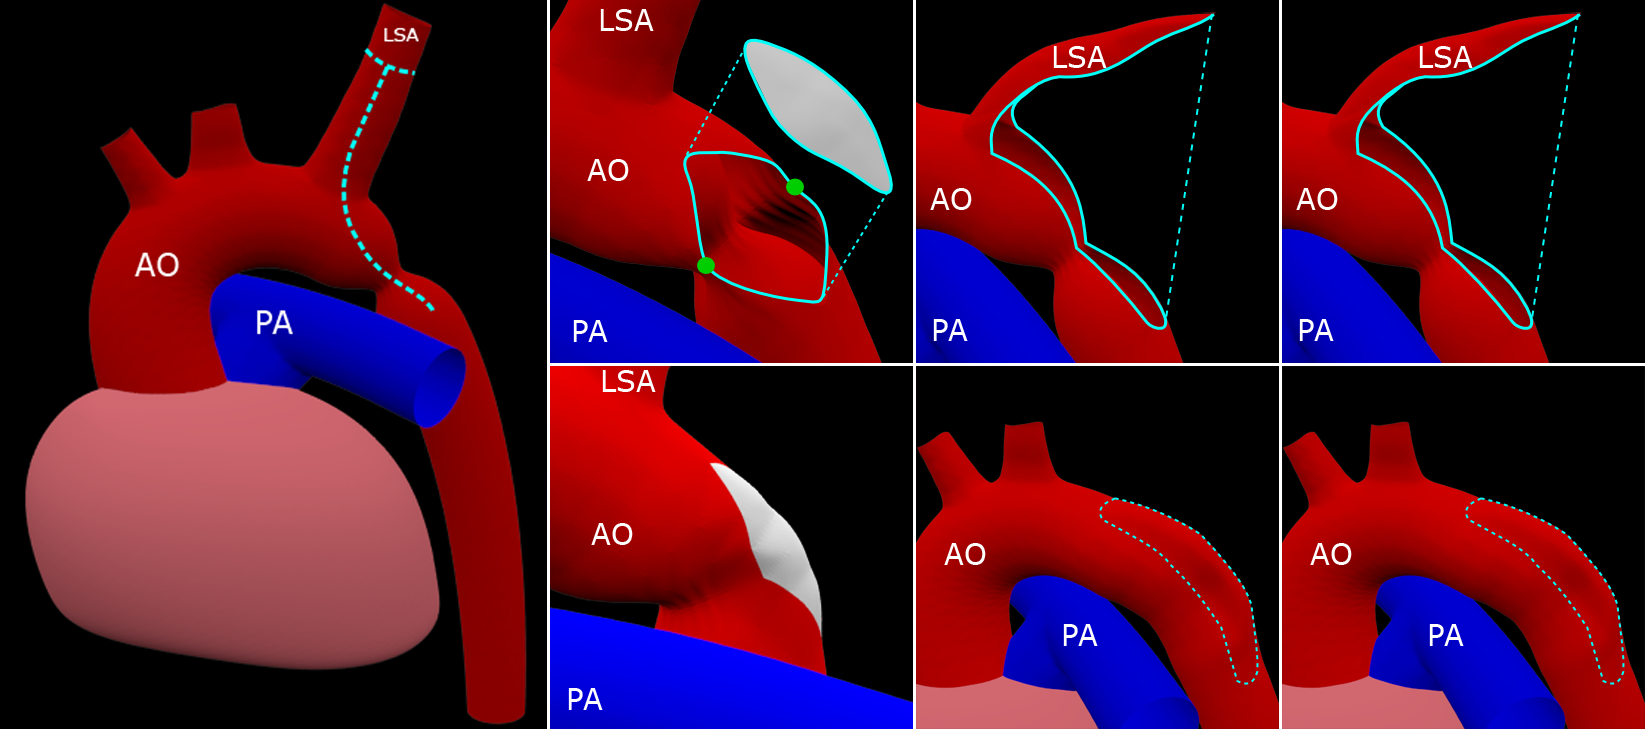
\includegraphics[width=\columnwidth]{img/surgery.png}
  \label{fig-surgery}
  \caption{Simulation of different surgical procedures for coarctation repair of an aortic arch. Left image: Overview of the simulation scene consisting of an aortic arch (AO), a left subclavian artery (LSA) and a pulmonary artery (PA). The coarctation can be seen next to the LSA and the dashed line indicates where the aorta is to be incised for a subclavian flap aortoplasty; The vertical image pairs show the scene before and after different surgical interventions. From left to right: Subclavian flap aortoplasty -- the subclavian flap is used as an organic onlay patch over the area of coarctation; Patch aortoplasty -- the incision is opened by attached springs only for visualisation purposes. The patch is sutured in place as shown; End-to-end anastomosis -- the coarctation is resected and the loose ends of th AO sutured together. Due to deformation of the AO it collides with the PA, causing a slight deformation there as well. }
\end{figure}

We manually modeled an aortic arch based on real image data to be able to demonstrate suitability of our joining approach for different kinds of low-level surgical procedures on a concrete example. Therefore we chose a coarctation of an aortic arch that can be repaired by completely different surgical approaches that heavily alter the surface of the blood vessel \cite{Dodge2000}. Results can be examined in figure \ref{fig-surgery}. We prove that our topological method for joining of shell elements through a controlled relaxation to their rest shape is able to handle all different kinds of connections universally and in a correct manner.

\subsection{Limitations and Constraints}
\tomas{rename do "Discussion"}

More general problems for this kind of simulation: (not limited to our method)

-- getting image data -- that is something you're already working on in Germany

-- hi-quality mesh with low number of polygons -- there seem to be something already, e.g. \cite{Comas2010c}.

At the moment biggest limitation of our method resides in the requirement of the same number of nodes on both edges of the suture.
Meeting this requirement may not be easy.
Also FE methods put constrain on the quality of mesh that is necessary to maintain the convergence and stability of the model.
These are especially important for meshes with low number of elements.
To deal with this problems techniques for dynamic remeshig during the simulation may be required.


%Example with 3 diff. surgical procedures
%Parameters
%Limitations (getting image data, meshes, dynamic remeshing, same number of nodes)
